% Figure from MATH 556 notes, section 15. Compile with the notes preamble.
\begin{tikzpicture}[scale=1.6, >=stealth]
    \draw[thick] (-1.3,0) -- (2.7,0) node[right] {$Y$};
    \draw[dashed, red!75!black] (-1.3,0.5) -- (2.7,0.5);
    \node[left, red!75!black] at (-1.3,0.5) {distance $\tfrac12$};
    \fill (0,0) circle (1.1pt) node[below] {$0$};
    \coordinate (X0) at (2.0,1.3);
    \coordinate (Y0) at (1.1,0);
    \fill (X0) circle (1.4pt) node[above right] {$x_0$};
    \draw[dashed, gray] (X0) -- (2.0,0) node[midway, right] {$d$};
    \fill (Y0) circle (1.3pt) node[below] {$y_0$};
    \draw[->, thick] (Y0) -- (X0) node[midway, left, xshift=-2pt] {$x_0 - y_0$};
    \draw[dotted, gray] (45:1) arc (45:100:1);
    \draw[->, thick, red!75!black] (0,0) -- (0.570,0.823) node[midway, left, red!75!black] {$z$};
    \node[gray!60!black] at (-0.55,1.02) {$\|z\| = 1$};
\end{tikzpicture}
